% ==========================================
% ТЕМАТИЧЕСКИЙ БАНК: МОМЕНТ СИЛЫ. СТАТИКА
% ВАРИАНТЫ 1-9 (ЕГЭ-2026, ДЕМИДОВА)
% ==========================================

\begin{taskbasic}[code={\label{task:statics_v01_n04}}]
\textbf{Задача 4.} Школьник выполнял лабораторную работу по исследованию условий равновесия лёгкого рычага под действием двух сил. Полученные результаты он занёс в таблицу.

\begin{center}
\begin{tabular}{|c|c|c|c|}
\hline
$F_{1}$, Н & $l_{1}$, м & $F_{2}$, Н & $l_{2}$, м \\ \hline
40 & 0{,}6 & 120 & ? \\ \hline
\end{tabular}
\end{center}

Каково плечо $l_{2}$, если рычаг находится в равновесии?

\kim{4}
\end{taskbasic}
\answer{0,2}

\begin{taskbasic}[code={\label{task:statics_v01_n26}}]
\textbf{Задача 26.} Тонкий однородный стержень $AB$ постоянного сечения шарнирно закреплён в точке $A$ и удерживается горизонтальной нитью $BC$, угол наклона стержня к горизонту $\alpha = 45^{\circ}$. Трение в шарнире пренебрежимо мало. Найдите массу стержня $m$, если модуль силы $F$, с которой шарнир действует на стержень, равен 35~Н. Сделайте рисунок, на котором укажите все силы, действующие на стержень. Обоснуйте применимость законов, используемых для решения задачи.
\nopagebreak\smallskip
\begin{center}
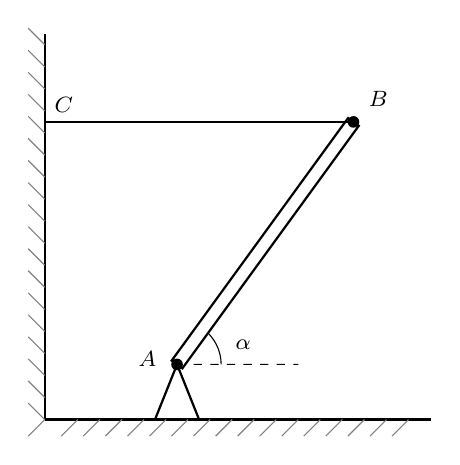
\begin{tikzpicture}[scale=1.4, every node/.style={font=\footnotesize}]
    % --- ГЕОМЕТРИЯ ОПОРНЫХ ПОВЕРХНОСТЕЙ ---
    % Вертикальная стена
    \draw[thick] (0,0) -- (0,3.5);
    \foreach \y in {0.0, 0.2,0.4,0.6,0.8,1.0,1.2,1.4,1.6,1.8,2.0,2.2,2.4,2.6,2.8,3.0,3.2,3.4}
        \draw[gray, thin] (0,\y) -- (-0.15,\y+0.15);
        
    % Горизонтальный пол
    \draw[thick] (0,0) -- (3.5,0);
    \foreach \x in {0.3,0.5,0.7,0.9,1.1,1.3,1.5,1.7,1.9,2.1,2.3,2.5,2.7,2.9,3.1,3.3}
        \draw[gray, thin] (\x,0) -- (\x-0.15,-0.15);
    
    % Угловая штриховка в начале координат
    \draw[gray, thin] (0,0) -- (-0.15,-0.15);



    % --- КОРЕННЫЕ ТОЧКИ (КООРДИНАТЫ) ---
    \coordinate (A) at (1.2,0.5);   % Шарнир стержня
    \coordinate (B) at (2.8,2.7);   % Верхний конец стержня
    \coordinate (C) at (0,2.7);     % Точка крепления нити на стене
% --- ОБОЗНАЧЕНИЕ УГЛА ALPHA ---
    % Пунктирный горизонт от точки А
    \draw[dashed, thin] (A) -- (2.3,0.5);
    % Дуга угла
    \draw (1.6,0.5) arc (0:54:0.4); % Угол наклона стержня примерно 54 градуса
    \node at (1.8,0.68) {$\alpha$};
% --- СТЕРЖЕНЬ AB ---
    % Отрисовка объемного стержня прямоугольником со скругленными краями через поворот
    \begin{scope}[shift={(A)}, rotate={atan2(2.7-0.5, 2.8-1.2)}]
        \draw[thick, fill=white] (0,-0.06) rectangle (2.72,0.06); % Длина стержня ~2.72
    \end{scope}
    % Точка B на конце стержня
    \fill[black] (B) circle (1.5pt) node[above right=2pt] {$B$};

    % --- ШАРНИРНАЯ ОПОРА А ---
    \draw[thick] (1.0,0) -- (A) -- (1.4,0);
    \fill[black] (A) circle (1.5pt) node[left=4pt, yshift=2pt] {$A$};

    

    % --- ГОРИЗОНТАЛЬНАЯ НИТЬ BC ---
    \draw[thick] (C) -- (B);
    \node[above right] at (C) {$C$};

    

\end{tikzpicture}
\end{center}
\kim{26}
\end{taskbasic}
\answer{5}

\begin{taskbasic}[code={\label{task:statics_v02_n04}}]
\textbf{Задача 4.} Школьник выполнял лабораторную работу по исследованию условий равновесия лёгкого рычага под действием двух сил. Полученные результаты он занёс в таблицу.

\begin{center}
\begin{tabular}{|c|c|c|c|}
\hline
$F_{1}$, Н & $l_{1}$, м & $F_{2}$, Н & $l_{2}$, м \\ \hline
80 & ? & 120 & 0{,}2 \\ \hline
\end{tabular}
\end{center}

Каково плечо $l_{1}$, если рычаг находится в равновесии?

\kim{4}
\end{taskbasic}
\answer{0,3}

\begin{taskbasic}[code={\label{task:statics_v02_n26}}]
\textbf{Задача 26.} Тонкий однородный стержень $AB$ постоянного сечения массой 2{,}7~кг шарнирно закреплён в точке $A$ и удерживается горизонтальной нитью $BC$, угол наклона стержня к горизонту $\alpha = 45^{\circ}$. Трение в шарнире пренебрежимо мало. Найдите модуль силы $F$, с которой шарнир действует на стержень. Сделайте рисунок, на котором укажите все силы, действующие на стержень. Обоснуйте применимость законов, используемых для решения задачи.
\nopagebreak\smallskip
\begin{center}
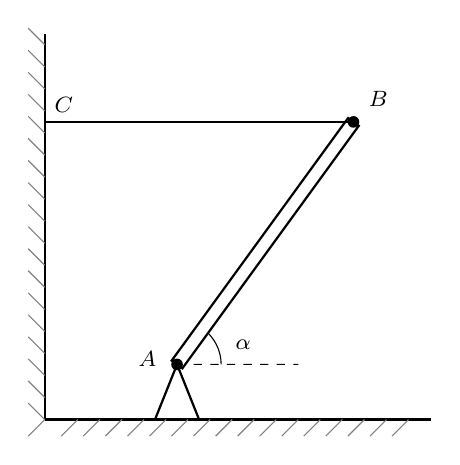
\begin{tikzpicture}[scale=1.4, every node/.style={font=\footnotesize}]
    % --- ГЕОМЕТРИЯ ОПОРНЫХ ПОВЕРХНОСТЕЙ ---
    % Вертикальная стена
    \draw[thick] (0,0) -- (0,3.5);
    \foreach \y in {0.0, 0.2,0.4,0.6,0.8,1.0,1.2,1.4,1.6,1.8,2.0,2.2,2.4,2.6,2.8,3.0,3.2,3.4}
        \draw[gray, thin] (0,\y) -- (-0.15,\y+0.15);
        
    % Горизонтальный пол
    \draw[thick] (0,0) -- (3.5,0);
    \foreach \x in {0.3,0.5,0.7,0.9,1.1,1.3,1.5,1.7,1.9,2.1,2.3,2.5,2.7,2.9,3.1,3.3}
        \draw[gray, thin] (\x,0) -- (\x-0.15,-0.15);
    
    % Угловая штриховка в начале координат
    \draw[gray, thin] (0,0) -- (-0.15,-0.15);



    % --- КОРЕННЫЕ ТОЧКИ (КООРДИНАТЫ) ---
    \coordinate (A) at (1.2,0.5);   % Шарнир стержня
    \coordinate (B) at (2.8,2.7);   % Верхний конец стержня
    \coordinate (C) at (0,2.7);     % Точка крепления нити на стене
% --- ОБОЗНАЧЕНИЕ УГЛА ALPHA ---
    % Пунктирный горизонт от точки А
    \draw[dashed, thin] (A) -- (2.3,0.5);
    % Дуга угла
    \draw (1.6,0.5) arc (0:54:0.4); % Угол наклона стержня примерно 54 градуса
    \node at (1.8,0.68) {$\alpha$};
% --- СТЕРЖЕНЬ AB ---
    % Отрисовка объемного стержня прямоугольником со скругленными краями через поворот
    \begin{scope}[shift={(A)}, rotate={atan2(2.7-0.5, 2.8-1.2)}]
        \draw[thick, fill=white] (0,-0.06) rectangle (2.72,0.06); % Длина стержня ~2.72
    \end{scope}
    % Точка B на конце стержня
    \fill[black] (B) circle (1.5pt) node[above right=2pt] {$B$};

    % --- ШАРНИРНАЯ ОПОРА А ---
    \draw[thick] (1.0,0) -- (A) -- (1.4,0);
    \fill[black] (A) circle (1.5pt) node[left=4pt, yshift=2pt] {$A$};

    

    % --- ГОРИЗОНТАЛЬНАЯ НИТЬ BC ---
    \draw[thick] (C) -- (B);
    \node[above right] at (C) {$C$};

    

\end{tikzpicture}
\end{center}
\kim{26}
\end{taskbasic}
\answer{25}

\begin{taskbasic}[code={\label{task:statics_v03_n26}}]
\textbf{Задача 26.} Однородный рычаг $AB$ может вращаться без трения вокруг неподвижной оси, проходящей через рычаг в точке $O$ перпендикулярно ему. К левому концу рычага в точке $A$ прикреплена нить, за которую с помощью динамометра $D$ рычаг неподвижно удерживается в горизонтальном положении. Нить составляет с вертикалью угол, который можно измерить с помощью транспортира $T$. Показания динамометра (в ньютонах) и транспортира (в градусах) видны на фотографии. К точке $C$ с помощью другой невесомой нерастяжимой нити подвешена медная пластина. Рычаг, пластина, нить и динамометр расположены в вертикальной плоскости. Массами транспортира и нитей пренебречь. Определите массу медной пластины, если рычаг имеет массу 30~г. Сделайте рисунок, на котором укажите все силы, действующие на рычаг и пластину. Обоснуйте применимость законов, используемых для решения задачи.


    \begin{center}
        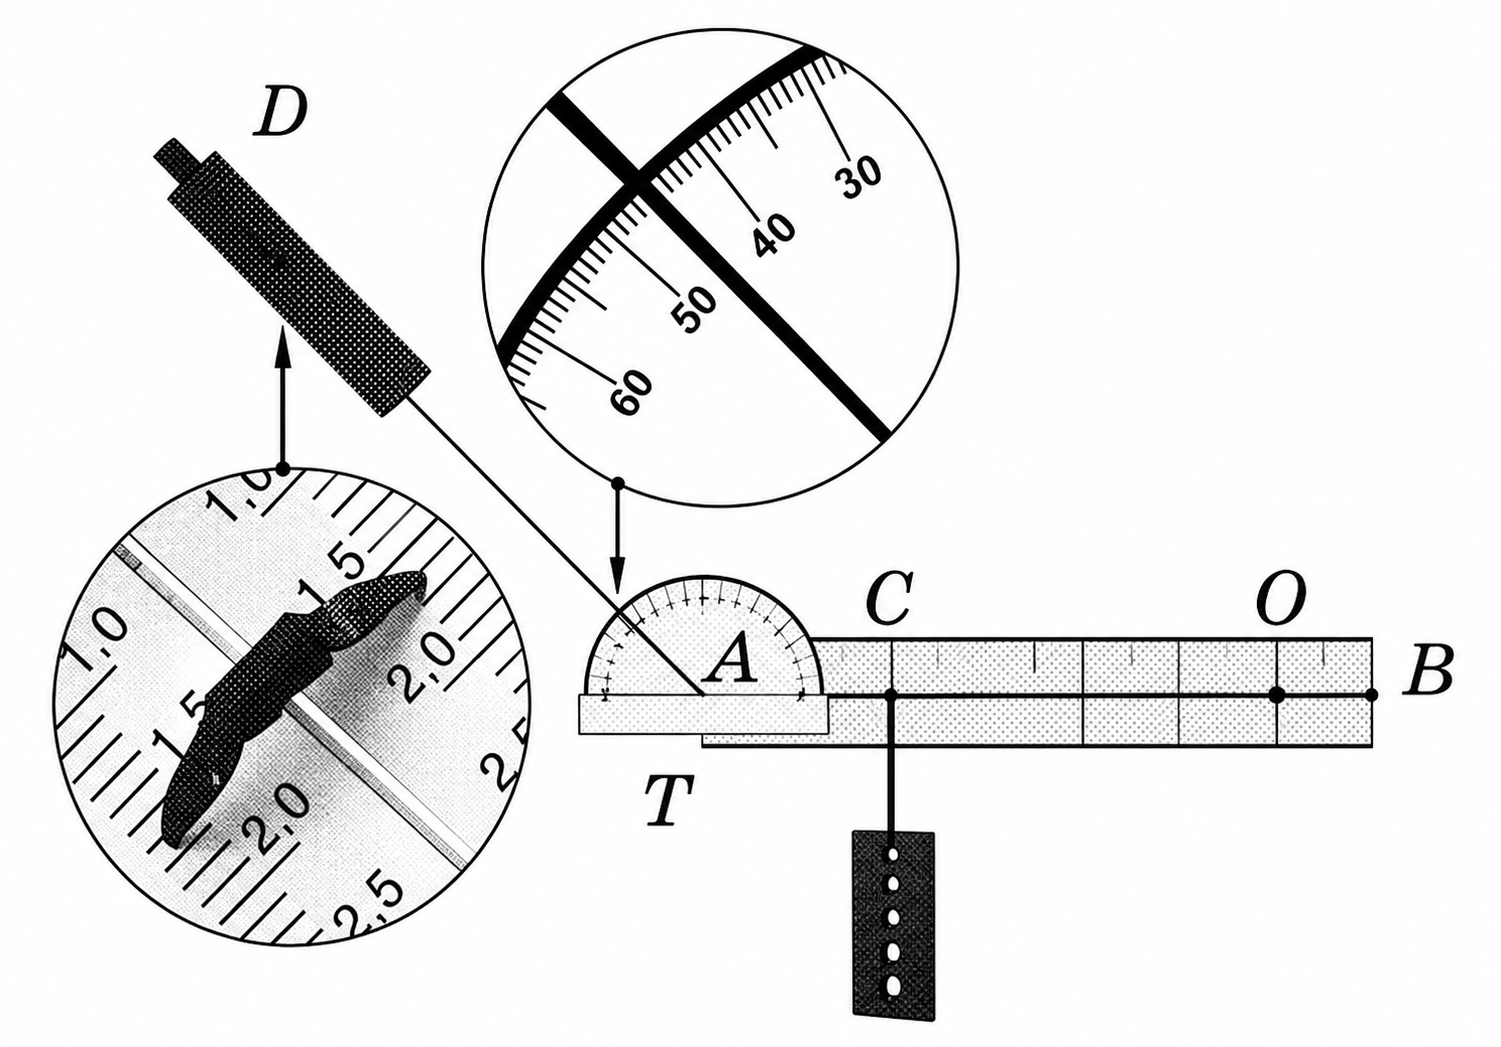
\includegraphics[width=0.5\linewidth]{01_mechanics/statics_1.png}
    \end{center}
    


\kim{26}
\end{taskbasic}
\answer{0,25}

\begin{taskbasic}[code={\label{task:statics_v04_n26}}]
\textbf{Задача 26.} Однородный рычаг $AB$ может вращаться без трения вокруг неподвижной оси, проходящей через рычаг в точке $O$ перпендикулярно ему. К левому концу рычага в точке $A$ прикреплена нить, за которую с помощью динамометра $D$ рычаг неподвижно удерживается в горизонтальном положении. Нить составляет с вертикалью угол, который можно измерить с помощью транспортира $T$. Показания динамометра (в ньютонах) и транспортира (в градусах) видны на фотографии. К точке $C$ с помощью другой невесомой нерастяжимой нити подвешена латунная пластина. Рычаг, пластина, нить и динамометр расположены в вертикальной плоскости. Массами транспортира и нитей пренебречь. Определите массу рычага, если латунная пластина имеет массу 120~г. Сделайте рисунок, на котором укажите все силы, действующие на рычаг и пластину. Обоснуйте применимость законов, используемых для решения задачи.

 \begin{center}
        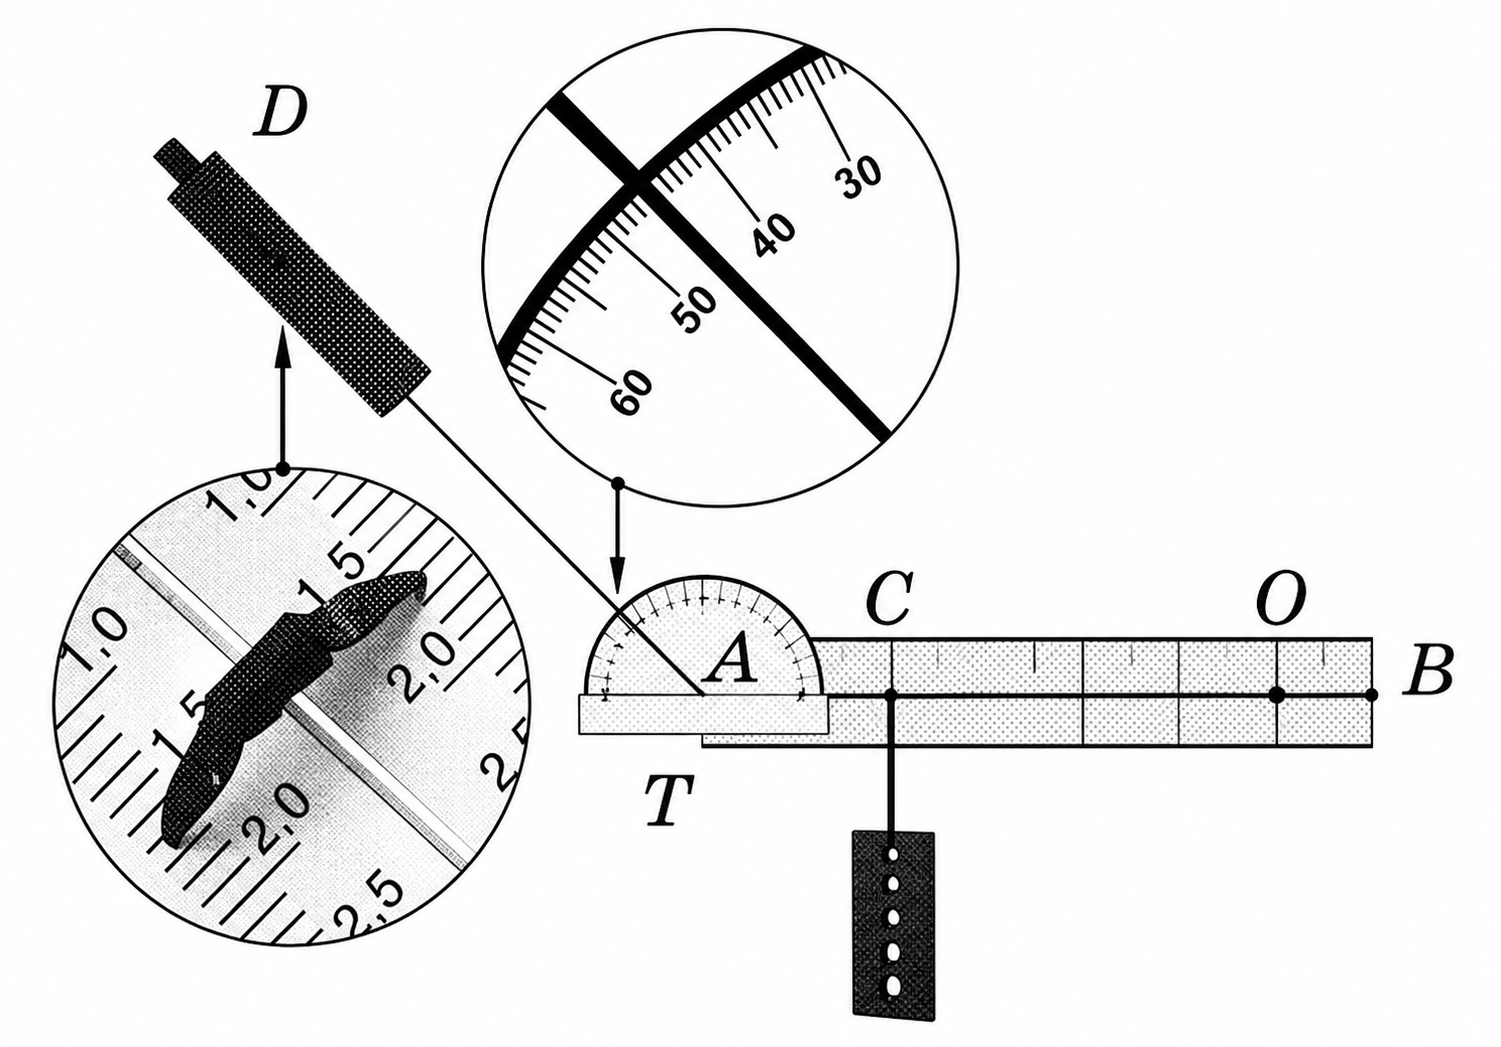
\includegraphics[width=0.5\linewidth]{01_mechanics/statics_1.png}
    \end{center}

\kim{26}
\end{taskbasic}
\answer{0,1}

% ==========================================
% ТЕМАТИЧЕСКИЙ БАНК: МОМЕНТ СИЛЫ. СТАТИКА
% ВАРИАНТЫ 5-9 (ЕГЭ-2026, ДЕМИДОВА)
% ==========================================

\begin{taskbasic}[code={\label{task:statics_v06_n26}}]
\textbf{Задача 26.} К концам невесомого рычага подвесили за невесомые нерастяжимые нити два сплошных груза массами $1{,}28$~кг и $0{,}32$~кг и привели рычаг в состояние равновесия. Затем рычаг с грузами расположили над водой так, что оба груза целиком оказались под водой. Первоначальное расстояние от более тяжёлого груза до точки опоры равно $20$~см. Определите, на сколько необходимо переместить точку опоры для сохранения равновесия, если объёмы обоих грузов одинаковы и равны $200$~\text{см}$^3$. Сделайте рисунок, на котором укажите силы, действующие на рычаг, для двух случаев, а также на погружённые в воду грузы. Обоснуйте применимость законов, используемых для решения задачи.

\kim{26}
\end{taskbasic}
\answer{0,22}

% ==========================================
% ТЕМАТИЧЕСКИЙ БАНК: МОМЕНТ СИЛЫ. СТАТИКА
% ВАРИАНТЫ 10-19 (ЕГЭ-2026, ДЕМИДОВА)
% ==========================================

\begin{taskbasic}[code={\label{task:statics_v11_n04}}]
\textbf{Задача 4.} Школьник выполнял лабораторную работу по исследованию условий равновесия лёгкого рычага под действием двух сил. Полученные результаты он занёс в таблицу.

\begin{center}
\begin{tabular}{|c|c|c|c|}
\hline
$F_{1}$, Н & $l_{1}$, м & $F_{2}$, Н & $l_{2}$, м \\ \hline
30 & 0{,}6 & 120 & ? \\ \hline
\end{tabular}
\end{center}

Каково плечо $l_{2}$, если рычаг находится в равновесии?

\kim{4}
\end{taskbasic}
\answer{0,15}

\begin{taskbasic}[code={\label{task:statics_v12_n04}}]
\textbf{Задача 4.} Школьник выполнял лабораторную работу по исследованию условий равновесия лёгкого рычага под действием двух сил. Полученные результаты он занёс в таблицу.

\begin{center}
\begin{tabular}{|c|c|c|c|}
\hline
$F_{1}$, Н & $l_{1}$, м & $F_{2}$, Н & $l_{2}$, м \\ \hline
60 & ? & 120 & 0{,}2 \\ \hline
\end{tabular}
\end{center}

Каково плечо $l_{1}$, если рычаг находится в равновесии?

\kim{4}
\end{taskbasic}
\answer{0,4}

% ==========================================
% ТЕМАТИЧЕСКИЙ БАНК: МОМЕНТ СИЛЫ. СТАТИКА
% ВАРИАНТЫ 10-19 (ЕГЭ-2026, ДЕМИДОВА)
% ==========================================

\begin{taskbasic}[code={\label{task:statics_v11_n04}}]
\textbf{Задача 4.} Школьник выполнял лабораторную работу по исследованию условий равновесия лёгкого рычага под действием двух сил. Полученные результаты он занёс в таблицу.

\begin{center}
\begin{tabular}{|c|c|c|c|}
\hline
$F_{1}$, Н & $l_{1}$, м & $F_{2}$, Н & $l_{2}$, м \\ \hline
30 & 0{,}6 & 120 & ? \\ \hline
\end{tabular}
\end{center}

Каково плечо $l_{2}$, если рычаг находится в равновесии?

\kim{4}
\end{taskbasic}
\answer{0,15}

\begin{taskbasic}[code={\label{task:statics_v12_n04}}]
\textbf{Задача 4.} Школьник выполнял лабораторную работу по исследованию условий равновесия лёгкого рычага под действием двух сил. Полученные результаты он занёс в таблицу.

\begin{center}
\begin{tabular}{|c|c|c|c|}
\hline
$F_{1}$, Н & $l_{1}$, м & $F_{2}$, Н & $l_{2}$, м \\ \hline
60 & ? & 120 & 0{,}2 \\ \hline
\end{tabular}
\end{center}

Каково плечо $l_{1}$, если рычаг находится в равновесии?

\kim{4}
\end{taskbasic}
\answer{0,4}

\begin{taskbasic}[code={\label{task:statics_v13_n26}}]
\textbf{Задача 26.} Два сплошных груза массами $1{,}28$~кг и $0{,}32$~кг подвесили за невесомые нерастяжимые нити к концам невесомого рычага и привели рычаг в состояние равновесия. Затем рычаг с грузами расположили над керосином так, что оба груза целиком оказались в керосине. В результате для сохранения равновесия точку опоры пришлось переместить на $10$~см. Определите первоначальное расстояние от более тяжёлого груза до точки опоры, если объёмы обоих грузов одинаковы и равны $250$~\text{см}$^3$. Сделайте рисунок, на котором укажите силы, действующие на рычаг, для двух случаев, а также на погружённые в керосин грузы. Обоснуйте применимость законов, используемых для решения задачи.

\kim{26}
\end{taskbasic}
\answer{22}

\begin{taskbasic}[code={\label{task:statics_v14_n26}}]
\textbf{Задача 26.} Два сплошных груза массами $1{,}28$~кг и $0{,}32$~кг подвесили за невесомые нерастяжимые нити к концам невесомого рычага и привели рычаг в состояние равновесия. Затем рычаг с грузами расположили над керосином так, что оба груза целиком оказались в керосине. В результате для сохранения равновесия точку опоры пришлось переместить на $10$~см. Определите первоначальное расстояние от более тяжёлого груза до точки опоры, если объёмы обоих грузов одинаковы и равны $250$~\text{см}$^3$. Сделайте рисунок, на котором укажите силы, действующие на рычаг, для двух случаев, а также на погружённые в керосин грузы. Обоснуйте применимость законов, используемых для решения задачи.

\kim{26}
\end{taskbasic}
\answer{25}